\chapter{States, Actions, Rewards}\label{sec:design}

\begin{figure}\centering
\begin{minipage}{.45\textwidth}
 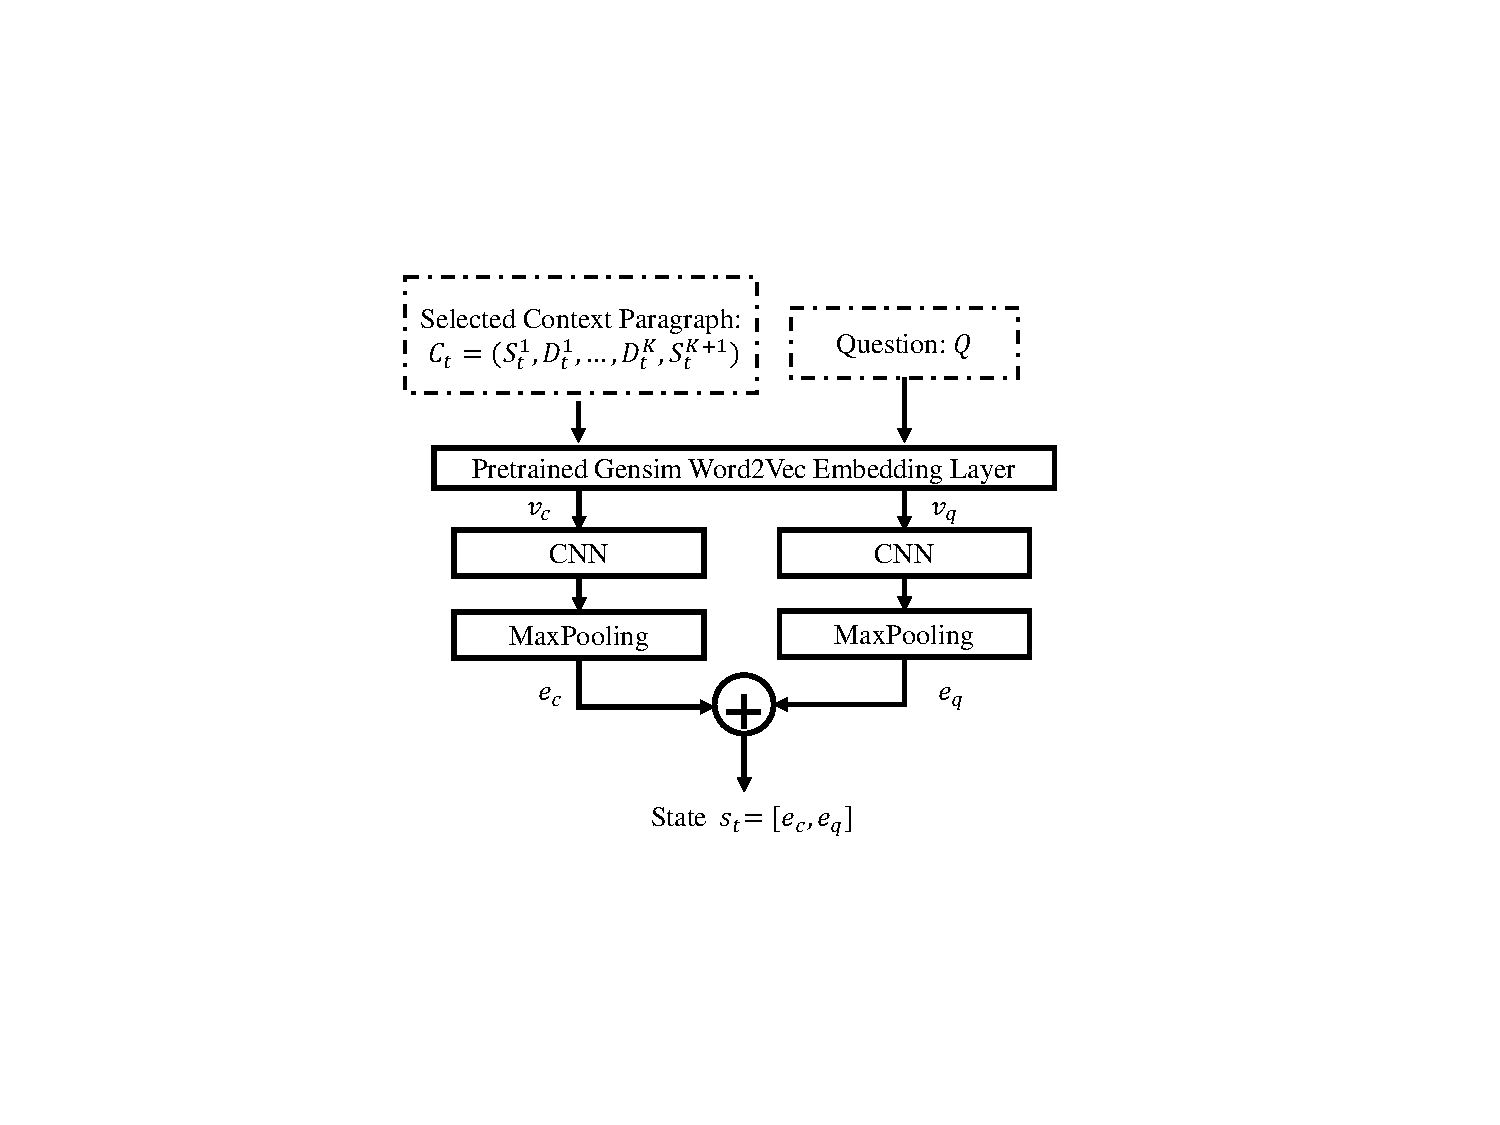
\includegraphics[width=0.9\linewidth]{Images/fig1_2.pdf}
 \caption{SGM Diagram}
 \label{fig:sgmDiagram}
\end{minipage}
\vspace{-2ex}
\end{figure}

\textbf{Design of State:} As our system's input, a state contains the information from both the context and the question (as shown in Figure \ref{fig:sgmDiagram}). %we designed state generation model (SGM) to generate their embeddings in order to construct the defined states. First, we train a preliminary word embedding dictionary using the gensim word2vec on a given dataset. By using these pre-trained word embeddings, 
We feed the context paragraph and the question separately into our state generation module (SGM), which contains an embedding layer and a convolutional layer followed by a max-pooling layer. The obtained embedding of the context paragraph is concatenated with that of the given question, in order to form a state as the input to RGM. The embedding layer is pre-trained using our dataset; the CNN and max-pooling layers are trained and updated together with our RL model. %, whose outputs are the actions to be defined in next section. Using this two-step approach, we can both leverage the fixed word-level information from our corpus and learn-able embedding information guided by the expected rewards obtained in DRL. %\kechen{add why we don't use coattention and intuition of choosing CNN}
%\subsection{Design of Actions}\label{design_action}
 %As defined in section XXX, t
 
 \textbf{Design of Actions:} The actions determine the reading focus at next time-step $t+1$. 
 % The design of actions is supposed to be close to one type of our human reasoning behaviors: using discourse markers and question topic to guide reading.
 Two different set of action designs are introduced as follows:
 
{\bf{ \underline{Action Set $1$:}}}
The first set of actions is designed only using the discourse markers, such that for each action, either context paragraph before or after a marker is chosen to be focused. An action is supposed to contain two pieces of information: (a) the word marker to be selected, and (b) the focus of reading from the selected marker, \emph{i.e. left} or \emph{right}. The action space is defined as $\lbrace\alpha_{1}^{left},\alpha_{1}^{right}, \cdots,\alpha_{k}^{left},\alpha_{k}^{right}\rbrace$, where $k$ discourse markers are selected from our discourse marker lexicon. The entire action space dimension is $\mathbb{R}^{2\times k}$ by considering the left and right directions. %After choosing an action, for example $\alpha_{i}^{left}$, the system will focus on the context \emph{left} to the discourse marker $d_{i}$, and vice versa for $\alpha_{i}^{right}$.

%\vspace{-1.0mm}
%\begin{itemize}[itemsep=0.1mm]
%\item The word marker to be selected.
%\item The focus of reading from the selected marker, \emph{i.e.} left or right.
%\vspace{-1.0mm}
%\end{itemize}
%In our model, we use the discourse marker, which is a main type of connectives, as the word markers described before. 

%which divide a document into multiple sentences/phrase segments. As in XXX, a human reader would like to use a word marker for reasoning in a machine reading task, %\cheng{I am not sure there is how humans read. I am not sure that the reviewers will buy this argument. Is there any behavior or psychological study that shows humans search for answers this way?} 
%Assuming that our system wants to imitate this learning process, our system's 
%Inspired by the work in XXX, in our model, we use the discourse markers, which is a main type of connectives, as the word markers for the model to select in this type of action design. 
%Furthermore, we also use the combination of discourse markers and target word(s) to define our action as shown in the second type of action design. \cheng{This is repeated in earlier sections}

%Also, in order to limit the action space size, we only select top $k$ discourse markers from XXX ranked by their frequencies in our datasets. By considering the searching directions from the selected discourse marker(s), the action space size is $2\times k$, which is the double of number of discourse markers selected. 
%A graphical illustration is as shown in Figure XXX:

%The action space includes $2\times k$ actions. At each time step $t$, the system selects one of them as the output of our DRL model. Specifically in our case, the DRL model will generate an action vector with a size of $2\times k$, where one of numbers in the vector is 1, and all the others are equal to 0s\kechen{why is that?}.


 {\bf{\underline{Action Set $2$:}}} The second set of actions leverages the information from both the discourse markers and the question topic. In our work, a target word is extracted from the question to capture question topic information. %By adding one more piece of information indicating the user's intention, 
 We expect that this action type can give better reasoning performance by associating the discourse information in context with the topic in question. The action space is defined as $\lbrace\alpha_{1}^{target},\alpha_{1}^{target\_{rev}}, \cdots,\alpha_{k}^{target},\alpha_{k}^{target\_{rev}}\rbrace$. After selecting an action $\alpha_i^{target}$, the system will focus on the text towards the direction to the target word from the discourse marker $d_i$ by ignoring the the text in the reverse direction; otherwise if action $\alpha_i^{target\_{rev}}$ is selected, the system will focus the text in the reverse direction to the target word from the discourse marker $d_i$, by ignoring the text in the same direction to the target word. For example, $\alpha_{ind(``until")}^{target\_{rev}}$ is selected in reasoning step 1 in Figure \ref{fig:qa_example} with the target word ``reheating", where $ind(*)$ returns the index of a word. It is worth noticing that if the same marker appears twice in a  selected context, the marker which is closer to the target word is picked.
 %\kechen{kechen add some intuition and entropy result}
%The action space is as shown in figure XXX.

 %To help better understand these action definitions, we also use an example to explain each action operation as in Figure XXX. \kechen{kechen add example}
 
 %\subsection{Design of Rewards}
\textbf{Design of Rewards:} 
% Another important element in reinforcement learning is the reward $r_t$, which can greatly affect the performance and robustness of a DRL model. In our system,
The reward $r_t$ is defined as whether the predicted segment $S'$ is the same as ground truth $S^*$ or not.
If it is, the reward is 1, otherwise it is 0. It is also worth noticing that the reward is only assigned to the final state, \emph{i.e.} no further action(s) to be performed for that context paragraph. The reward at other time-steps is 0.

%In our scenario, the ground truth $A^*$ is the correct answer given a context and a question. 

%\kechen{2.6 is incomplete? In particular, I need more information to understand the objective functions in equation 1.}
 % In this work, we use the actor-critic based algorithm  to build our DRL model. %Unlike the value based DRL approach like DQN \cite{mnih2015human} or policy based approach like policy gradient \cite{sutton2000policy}, an actor-critic based model has a better performance on continuous state space in terms of convergence and stability.
 % Due to the space limitation and the focus of this paper, we will only describe the actor-critic method briefly.
%\subsubsection{Training}

In an Actor-Critic based DRL algorithm, two separate neural networks are built to model the actor and critic. The actor updates the policy parameters $\theta$ for $\pi_\theta(a_t|s_t)$, while the critic predicts an expected reward at that state to assist the policy update. %The actor model performs like a policy gradient approach \cite{sutton2000policy} by taking state $s_t$ as its input and generating action probabilities based on the policy: $\pi_\theta(a_t|s_t)$. Comparatively, the critic model applies a value based algorithm, like $DQN$ \cite{mnih2015human}. 
At each training iteration, by performing the action $a_t$ generated by actor, the system transits to a new state $s_{t+1}$ from its current state $s_t$, and then the critic  can generate two values (\emph{i.e.} expect rewards) $v_t$ and $v_{t+1}$ by taking $s_t$ and $s_{t+1}$ as inputs. There are two separate loss functions, training the actor and the critic models:
\begin{equation}
%\vspace{-0.5ex}
\begin{split}
\mathcal{L}_{actor}&=-\log \pi_{\theta} (a_t|s_t)(r_t+\gamma v_{t+1}-v_{t})\\
\mathcal{L}_{critic}&=(r_t+\gamma v_{t+1}-v_{t})^2
\label{rlloss}
\end{split}
\end{equation}
where $\gamma$ is a discount factor in our DRL model. From the loss function, we can see that the actor model aims to maximize the expected rewards to be obtained, and the critic model minimizes the temporal difference error during the stochastic learning process. Compared to the commonly used policy-gradient RL algorithm, an actor-critic based model has a better performance in terms of convergence and stability. During inference, our model reads in a sample containing the full context paragraph $C_0$ and question $Q$. At each time step $t$, the model generates an action which leads to a new context paragraph $C_{t+1}\subset C_t$. This inference process stops when there is no discourse marker contained in the current context paragraph, which is also the final predicted segment $S^{\prime}$ as in Figure \ref{fig:systemDiagram}. During training and inference, if the selected discourse marker does not appear in the context, the model will do the selection again.